% !TEX root = ../main.tex
%
\chapter{Verwandte Arbeiten}
\label{sec:related}

Die in~\ref{sec:intro:goals} beschriebenen Ziele werden bereits seit langem erforscht.
Der Begriff \textit{Wissensgraph} wurde 2012 durch Google popularisiert, die Ideen dahinter lassen sich allerdings bis ins Ende des 19. Jahrhunderts zurückverfolgen.
Dieses Kapitel zeigt auf, wie sich die Themen dieser Arbeit in die bisherige Forschung einfügen.
\ref{sec:related:kr} ordnet das Konzept des Wissensgraphen in die Entwicklungsgeschichte der Wissensrepräsentation ein.
\ref{sec:related:kbc} beschreibt die aktuell verwendeten Verfahren zur Konstruktion von Wissensgraphen.
In~\ref{sec:related:nlp} wird schließlich ein Überblick über die momentan verbreiteten NLP (\textit{natural language processing}) Werkzeuge gegeben.

\section{Ansätze zur Wissensrepräsentation}
\label{sec:related:kr}

\subsection{Logische Grundlagen}
\label{sec:related:kr:logic}

Die Entwicklung der Wissensrepräsentation hängt eng mit der Entwicklung der Logik zusammen.
Während in der formalen Logik und Mathematik die Prädikatenlogik das allgemein verwendete Kalkül ist und alternative Formalismen kaum verbreitet sind, finden im Bereich der Wissensrepräsentation bis heute diverse andere Kalküle Verwendung.
Diese werden im Folgenden kurz vorgestellt.

\paragraph{Begriffsschrift (1879)}
Gottlob Freges Buch über die \textit{Begriffsschrift} gilt als eines der bedeutsamsten Werke der Logik.
Sie ist der erste Formalismus mit der Mächtigkeit der modernen Prädikatenlogik zweiter Ordnung mit Identität.
Frege benutzt hierfür eine zweidimensionale Notation, die sich stark von der heute gebräuchlichen, linearen, an die Algebra angelehnte Notation unterscheidet.
\begin{equation*}
	\vcenter{\hbox{\Fconditional[\Fanqn{a}]{\Fcontent \mathfrak{R(a)}}{\Fncontent \mathfrak{P(a)}}}}
	\quad\Leftrightarrow\quad
	\exists\ a: P(a) \lor R(a)
\end{equation*}
Im Gegensatz zur Prädikatenlogik gibt es keine eigene Syntax für \textit{UND} und \textit{ODER};
diese Operatoren müssen durch die Kombination von Negation und Implikation abgebildet werden.
Zudem gibt es ausschließlich den Allquantor;
eine existenzquantisierte Aussage muss durch Negation der negierten allquantisierten Aussage ausgedrückt werden.

\paragraph{Prädikatenlogik: Peirce Notation (1885)}
Unabhängig von Frege entwickelte der amerikanische Mathematiker Charles Sanders Peirce ebenfalls ein prädikatenlogisches Kalkül.
Peirces Notation hatte starke Ähnlichkeiten mit der heute benutzten linearen Schreibweise.
Statt den modernen Symbolen hat Peirce allerdings die algebraischen Operatoren benutzt, um die Analogien zwischen Logik und Algebra auszudrücken.
\begin{equation*}
	\Sigma_a\ P_a + R_a
	\quad\Leftrightarrow\quad
	\exists\ a: P(a) \lor R(a)
\end{equation*}

\paragraph{Existential Graphs (1897)}
Neben seiner zuvor entwickelten linearen prädikatenlogischen Notation, hat Peirce zudem viele Jahre an einem alternativen graphischen Kalkül gearbeitet, welches er \textit{Existential Graphs} (zu dt.~Existenzgraphen) nannte.
Ähnlich wie die Begriffsschrift werden Existenzgraphen zweidimensional dargestellt.
Von dieser Gemeinsamkeit abgesehen, funktionieren sie allerdings fundamental verschieden.
Ein logischer Ausdruck wird hier durch einen ungerichteten Graphen beschrieben.
Die konkrete räumliche Anordnung der Knoten und Kanten hat dabei keine semantische Relevanz.

Peirce hat Existenzgraphen als ein dreistufiges aufeinander aufbauendes System konzipiert.
Die erste Stufe, die sog.\ $\alpha$-Graphen, umfasst alle notwendigen syntaktischen Elemente, um ein Kalkül mit der Mächtigkeit der Aussagenlogik zu erhalten.
Die $\beta$-Graphen bilden die zweite Stufe und erweitern die Syntax der $\alpha$-Graphen, sodass die Mächtigkeit der Prädikatenlogik erster Ordnung erreicht wird.
Sowohl für $\alpha$-, als auch für $\beta$-Graphen, ist die Vollständigkeit und Korrektheit bewiesen.
Die dritte Stufe ($\gamma$-Graphen) wurde von Pierce nie vollendet;
sie deckt in etwa die Mächtigkeit der heutigen Prädikatenlogik höherer Ordnung sowie der Modallogik ab.
\begin{align*}
	\vcenter{\hbox{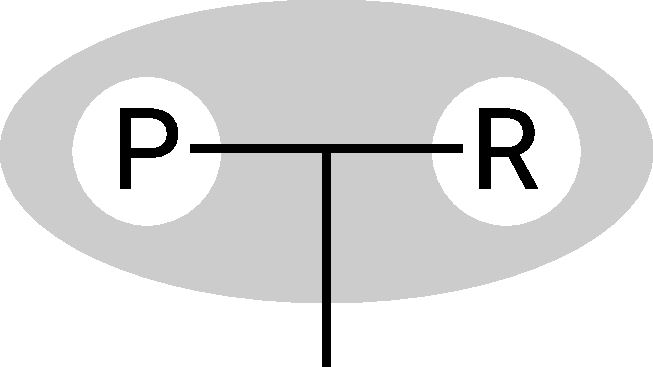
\includegraphics[height=3em]{gfx/related-work/existentialGraphExample1.pdf}}}
	\quad\Leftrightarrow\quad
	\exists\ a: P(a) \lor R(a)
\end{align*}
Wie schon die Begriffsschrift, sind Existenzgraphen syntaktisch minimal.
Direkt ausdrücken lässt sich lediglich \textit{UND}, der Existenzquantor und die Negation.
Ein weiterer Unterschied zur heutigen Prädikatenlogik ist die Beschreibung logischer Inferenzen.
Im Gegensatz zu den prädikatenlogischen Ersetzungsaxiomen, die auf der syntaktischen Struktur von logischen Ausdrücken operieren (z.~B. für Kommutativität), lassen sich die Ersetzungsaxiome für Existenzgraphen als Graphtransformationsregeln verstehen, die bestimmte Teilmengen der Knoten und Kanten eines Ausdrucks durch andere äquivalente Knoten- und Kantenmengen ersetzen.

\paragraph{Prädikatenlogik: Peano-Russell Notation (1910)}
Die zweidimensionalen Notationen wurde häufig kritisiert, da sie die lineare, algebraische Notation der symbolischen Logik von Boole und De Morgan verwarfen.
Freges Begriffsschrft und Peirces Existenzgraphen konnten sich daher nicht durchsetzen.
Peirces algebraische prädikatenlogische Notation hingegen, stieß auf größere Akzeptanz.
Giuseppe Peano hat auf deren Basis eine ähnliche Notation entwickelt, welche allerdings nicht die algebraischen Operatoren benutzt, damit sich logische Ausdrücke besser mit mathematischen Ausdrücken kombinieren lassen.
Bertrand Russell hat Peanos Notation anschließend in leicht abgewandelter Form in den \textit{Principia Mathematica} (1910) benutzt.
Diese sog.~Peano-Russell-Notation ist im Wesentlichen identisch mit der modernen Schreibweise.

Trotz des Verschwindens der zweidimensionalen Notationen, finden sich noch heute Anlehnungen daran.
So ist z.~B. die Negation $\lnot A$ auf Freges negierten Inhaltsstrich $\Fncontent A$ und der Ableitungsoperator $\vdash$ auf Freges Urteilsstrich mit angefügtem Inhaltsstrich $\Facontent$ zurückzuführen.

\subsection{Entwicklung maschineller Wissensrepräsentation}
\label{sec:related:kr:history}

Die Idee Computer zur Lösung beliebiger Probleme zu benutzen ist nicht neu.
Da ein solches maschinelles Problemlösen immer die Verfügbarkeit von Hintergrundwissen über die Problemdomäne erfordert,
wurden Methoden zur Wissensrepräsentation immer im Zusammenhang mit Problemlösern erforscht.
So wie effiziente Datenstrukturen die Implementation effizienter Algorithmen ermöglichen, ermöglichen gute Wissensrepräsentationen die Implementation guter Problemlöser.
Was genau nun als ein guter Problemlöser verstanden wird, hat sich im Laufe der Jahre allerdings immer wieder verändert.

\paragraph{Universelle Problemlöser}
Einer der ersten maschinellen Problemlöser war der von Simon, Shaw und Newell 1955 entwickelte \textit{Logic Theorist} (LT).
LT war in der Lage logische Aussagen zu beweisen, indem er systematisch Ersetzungsaxiome auf eine gegebene Aussage angewandt hat, bis die gesuchte Lösung abgeleitet wurde.

Die Grundidee des LT haben Simon, Shaw und Newell 1959 im \textit{General Problem Solver} (GPS) erweitert.
Es wurden Heuristiken hinzugefügt, um den Suchraum geschickter zu durchlaufen.
GPS war ein universeller Problemlöser, konnte also jedes Problem lösen, das sich durch eine Menge von Horn-Klauseln ausdrücken lässt.
Zwar war es so theoretisch möglich Probleme aus diversen Domänen zu lösen, aufgrund der kombinatorischen Explosion war GPS alledings nicht zur Lösung komplexer praktischer Probleme geeignet.

\paragraph{Expertensysteme}
Aufgrund der Misserfolge universeller Problemlöser für praktische Probleme, hat die Forschung begonnen sich mehr auf die Entwicklung von Expertensystemen zu fokussieren.
Expertensysteme besitzen für gewöhnlich eine Wissensbasis in der domänenspezifisches Wissen in Form von Regeln und Fakten kodiert ist.
Eine sog.~Inferenzmaschine benutzt diese Regeln und Fakten um Probleme zu lösen.

\paragraph{Semantic Networks (1956)}
Die Idee, Graphen als Datenstruktur für Wissensbasen zu verwenden, taucht erstmal in den sog.~\textit{Semantic Networks} (zu dt.~semantische Netzwerke) auf.
Dieser Ansatz beschreibt Wissen als Menge von $(subject, predicate, object)$-Tripeln.
Es gibt darüber hinaus keine klaren Regeln, wie ein semantisches Netz strukturiert sein muss.

\paragraph{Conceptual Graphs (1976)}
Wie genau mit Graphen komplexes Wissen beschrieben werden kann, das über eine reine Taxonomie hinaus geht, blieb bei semantischen Netzen unklar.
John F. Sowas \textit{Conceptual Graphs} (zu dt.~Konzeptgraphen) lösen dieses Problem.
Statt Wissen als eine Menge von Beziehungen abzubilden, wird es als prädikatenlogischer Ausdruck verstanden.
Hierfür baut Sowa auf Peirces Existenzgraphen auf, die bis dahin weitestgehend unbeachtet waren.
\begin{align*}
	\vcenter{\hbox{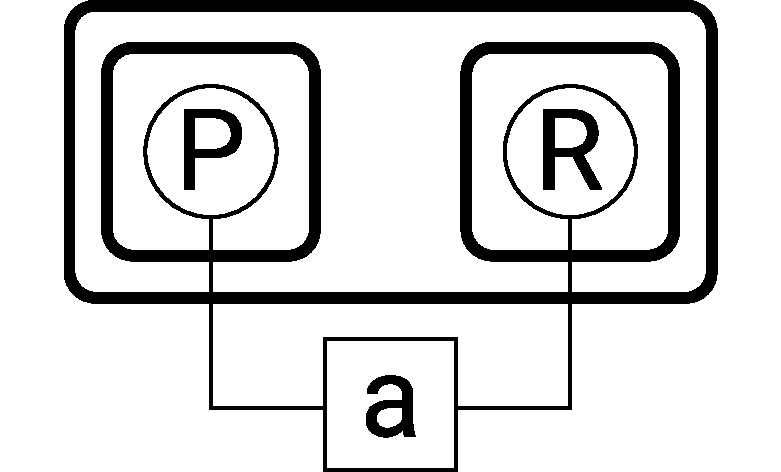
\includegraphics[height=4em]{gfx/related-work/conceptGraphExample1.pdf}}}
	\quad\Leftrightarrow\quad
	\exists\ a: P(a) \lor R(a)
\end{align*}
Dieser Ansatz erlaubt es komplexe Wissensbasen zu konstruieren, in denen nicht nur gespeichert werden kann, ob ein Konzept existiert, sondern auch, ob es nicht oder nur möglicherweise existiert.
Da Konzeptgraphen, so wie schon die Existenzgraphen, ein vollständiges und korrektes Logikkalkül sind, lassen sich zudem Inferenzregeln für sie definieren.
Der Vorteil hierfür einen Graphen statt eines prädikatenlogischen Ausdrucks zu verwenden ist, dass eine Graphstruktur einen deutlich effizienteren Zugriff auf gespeichertes Wissen ermöglicht.

\paragraph{Knowledge Graphs (1987)}
Der Begriff \textit{Knowledge Graph} (zu dt.~Wissensgraph) bezeichnete ursprünglich eine Klasse semantischer Netze, deren Relationsmenge formal spezifiziert ist.
Dies schränkt die Menge erlaubter Graphen ein und ermöglicht die Definition von Inferenzregeln, um Schlussfolgerungen aus einem gegebenen Graphen zu ziehen.
Im Laufe der Jahre ist die Grenze zwischen semantischen Netzen und Wissensgraphen allerdings immer weiter verschwommen, sodass die Bezeichnungen heute oft synonym verwendet werden.
Wissensgraphen und Konzeptgraphen müssen weiterhin unterschieden werden, da erstere oftmals Negation und Modalität nicht unterstützen.

\subsection{Aktuelle Wissensrepräsentationsprojekte}
\label{sec:related:kr:today}

\subsubsection{Manuelle Ansätze}

\paragraph{Semantic Web}
Das sog.~\textit{Semantic Web} bezeichnet eine Menge von W3C-Standards, die das bestehende Web um eine formale Wissensbeschreibungssyntax erweitern.
Zentral ist dabei das \textit{Resource Description Framework} (RDF), mit dem sich beliebige Konzepte, auch Resourcen genannt, beschreiben und verknüpfen lassen.
Ziel ist es über die unstrukturierte Netzstruktur des bestehenden Webs, eine strukturierte, leicht maschniell verarbeitbare, Netzstruktur zu legen.
Durch die Anfragesprache \textit{SPARQL} ist es möglich Wissen aus diesem Netz auszulesen.
Das Web würde somit zu einem großen denzentralen Wissensgraphen.
Tim Berners-Lee beschreibt diese Idee als das ``Web 3.0''.
Obwohl die Technologien hierfür bereits seit Jahren existieren, sind bislang nur wenige Webseiten mit RDF-Tags annotiert.
Häufige Kritik ist, dass das Semantic Web zu viel theoretisches Hintergrundwissen über Wissensrepräsentationsverfahren erfordert, um für die meisten Webseitenbetreiber zugänglich zu sein.

\paragraph{WordNet}
Das \textit{WordNet} der Universität Princeton ist ein frei verfügbares lexikalisch-semantisches Netz für die englische Sprache, d.~h.\ ein semantisches Netz, welches die Bedeutung von Worten in Relation zueinander setzt.
Relationen werden dabei z.~B. für Synonyme, Hypernyme (Oberbegriffe) und Meronyme (Bestandteile) eingefügt.
Der Datenbestand des WordNets wird manuell gepflegt und resultiert aus der Kombination der Einträge verschiedener Wörterbücher.

\subsubsection{Automatisierte Ansätze}
Neben den manuellen Grapherzeugungsansätzen des Semantic Webs und des WordNets, gibt es diverse voll- und semiautomatische Ansätze.
Diese bauen die Graphstruktur selbstständig aus gegebenen Datenquellen auf.

\paragraph{NELL}
Das \textit{Never-Ending Language Learning} (NELL) System traviersiert selbstständig das Internet und fügt die gefundenen textuellen Informationen in einen Wissensgraphen ein.
Hierfür wird eine Kombination verschiedener Modelle verwendet, die regelmäßig angepasst wird.
Menschen können optional Feedback für die extrahierten Fakten geben, um die Inferenzqualität weiter zu verbessern.

\paragraph{Google Knowledge Graph}
test

\begin{figure}
	\begin{tikzpicture}
		\pgfplotstableread[col sep=comma] {data/related-work/knowledgeGraph.csv}\knowledgeGraphTrend%
		\begin{axis}[
			width=\textwidth,
			height=6cm,
			smooth,
			axis x line=bottom,
			axis y line=left,
			axis lines=center,
			ymin=0,
			ymax=100,
			ylabel={Popularität in \%},
			date coordinates in=x,
			date ZERO=2004-01-01,
			xmin={2004-01-01},
			xmax={2017-08-01},
			xticklabel={\month.\year},
			xtick={2004-01-012,2012-05-01,2017-08-01}
		]
			\addplot+[no markers,style=thick] table [x=month, y=popularity]{\knowledgeGraphTrend};
		\end{axis}
	\end{tikzpicture}
	\caption{Relative Popularität des Suchbegriffs ``knowledge graph'' (Quelle: Google Trends)}\label{fig:related:kgTrend}
\end{figure}

{\sffamily Dies ist ein Roboto-Test 123.}

\section{Wissensgraphkonstruktionsverfahren}
\label{sec:related:kbc}

\section{NLP Werkzeuge}
\label{sec:related:nlp}
